\section{JC1 Promotional Examination - H2 Further Mathematics 9649}

\begin{problem}
    Given that $z = f(x, y)$ is a differentiable function and $f(x, y) = k$ is the level curve of $f$ that passes through the point $P$, show that the gradient vector $\nabla f$ is perpendicular to the tangent of the level curve at $P$.
\end{problem}
\begin{solution}
    Let $x$ and $y$ be parametrized $t$. Implicitly differentiating $f(x, y) = k$ with respect to $t$, we obtain \[\pder{f}{x} \der{x}{t} + \pder{f}{y} \der{y}{t} = 0 \implies \cvecii{\pderx{f}{x}}{\pderx{f}{y}} \dotp \cvecii{\derx{x}{t}}{\derx{y}{t}} = 0.\] Observe that $\cveciix{\pderx{f}{x}}{\pderx{f}{y}}$ is exactly $\nabla f$. Taking $t = x$, we also have $\cveciix{\derx{x}{t}}{\derx{y}{t}} = \cveciix{1}{\derx{y}{x}}$, which is the tangent vector of the level curve at $P$. Since the dot product of the two vectors is 0, they must be perpendicular.
\end{solution}

\begin{problem}
    A harvesting model is given by $\der{P}{t} = (20-P)\bp{P^2 - 30 P + h}$ where $P$ is the population of the resource at time $t$ and $h$ is the constant harvest rate. It is given that at $t = 0$, $P = 50$. Find the range of values of $h$ such that $P=20$ in the long run.
\end{problem}
\begin{solution}
    Let $f(P) = (20-P)\bp{P^2 - 30 P + h}$. For $P = 20$ in the long run, we need $f(P) < 0$ for all $P \in (20, 50]$. Observe that $20 -P < 0$ for all $P \in (20, 50]$. We hence need $P^2 - 30 P + h > 0$ for all $P \in (20, 50]$. However, observe that $P^2 - 30P + h$ is strictly increasing after $P > 15$. Thus, we only require the quadratic to be non-negative at $P = 20$, whence $20^2 - 30(20) + h \geq 0$, giving $h \geq 200$.
\end{solution}

\begin{problem}
    \begin{enumerate}
        \item Describe the locus given by $\abs{2\i + 1 + \i z} = \abs{4\i - 5 - z}$.

        $S$ is the set of complex numbers $z$ for which \[\abs{2\i + 1 + \i z} \geq \abs{4\i - 5 - z} \land \abs{z + 2 - 3\i} \leq \sqrt{13}.\]
        \item On a single Argand diagram, shade the region corresponding to $S$.
        \item Find the set of values of $\arg{z - 8\i}$.
    \end{enumerate}
\end{problem}
\begin{solution}
    \begin{ppart}
        Note that $\abs{2\i + 1 + \i z} = \abs{2 - \i + z} = \abs{z - (-2 + \i)}$. We hence have \[\abs{z - (-2 + \i)} = \abs{z - (-5 + 4\i)},\] which describes the perpendicular bisector of the line segment joining $(-2, 1)$ and $(-5, 4)$.
    \end{ppart}
    \clearpage
    \begin{ppart}
        \begin{center}\tikzsetnextfilename{1}
            \begin{tikzpicture}[trim axis left, trim axis right]
                \begin{axis}[
                    domain = 0:10,
                    samples = 101,
                    axis y line=middle,
                    axis x line=middle,
                    xtick = \empty,
                    ytick = {6, 8},
                    xmax=4,
                    xmin=-7,
                    ymin=-1,
                    ymax=8.5,
                    xlabel = {$\Re$},
                    ylabel = {$\Im$},
                    legend cell align={left},
                    legend pos=outer north east,
                    after end axis/.code={
                        \path (axis cs:0,0) 
                            node [anchor=north east] {$O$};
                        }
                    ]
        
                    \coordinate (R) at (10,0);
                    \coordinate[label=right:$\bp{-5, 4}$] (Z1) at (-5, 4);
                    \coordinate[label=below:$\bp{-2, 1}$] (Z2) at (-2, 1);
                    \coordinate[label=below:$\bp{-2, 3}$] (Z3) at (-2, 3);
                    \coordinate (O) at (0, 0);

                    \draw (-2, 3) circle[radius=sqrt(13)];
            
                    \draw[dashed] (Z1) -- (Z2);
                    \draw (-7, -1) -- (4, 10);
            
                    \fill (Z1) circle[radius=2.5pt];
                    \fill (Z2) circle[radius=2.5pt];
                    \fill (Z3) circle[radius=2.5pt];

                    \draw[dotted] (Z3) -- (1.6056, 3);

                    \node[anchor=south] at ($(Z3)!0.75!(1.6056, 3)$) {$\sqrt{13}$};

                    \node[anchor=east] at (-5, 6) {$S$};
                    \draw[->] (-5.1, 5.9) -- (-4, 5);
                \end{axis}
            \end{tikzpicture}
        \end{center}
    \end{ppart}
    \begin{ppart}
    Clearly, $\min \arg(z- 8\i) = -\frac\pi2$ (where $z = 6\i$). Let $A(-2, 3)$ and $B(0, 8)$. Let $C$ be the point on the circle such that $BC$ is tangent to the circle. We have $\angle ABO = \arctan \frac{2}{5}$. Since $AB = \sqrt{5^2 + 2^2} = \sqrt{29}$, we also have $\angle CBA = \arcsin \frac{\sqrt{13}}{\sqrt{29}}$. Thus, \[\max \arg{z - 8\i} = -\frac\pi2 - \arctan \frac{2}{5} - \arcsin \frac{\sqrt{13}}{\sqrt{29}} = -2.68,\] whence \[-2.68 \leq \arg{z-8\i} \leq -\frac\pi2.\]
    \end{ppart}
\end{solution}

\begin{problem}
    A tuition agency is designing a revision programme to help students to prepare for their A-level examinations. There are three types of revisions that the agency can run each day: Basic, Intermediate and Challenging. Due to resource constraints, the Challenging revision cannot be run consecutively. The revision programme consists of $n$ days. Let $a_n$ be the number of possible programmes for the duration.

    \begin{enumerate}
        \item Explain why $a_n = 2(a_{n-1} + a_{n-2})$.
        \item Solve the recurrence relation and find $a_n$ in terms of $n$.
        \item For a 10 days revision programme, given that both the 1st and 10th days consist of the Challenging revision, find the number of possible programmes.
    \end{enumerate}
\end{problem}
\begin{solution}
    \begin{ppart}
        Suppose the $n$th day ran Basic or Intermediate. The agency was hence free to run any programme on the $n-1$th day, thus contributing $2 \cdot a_{n-1}$ total programmes towards $a_n$.

        Now suppose the $n$th day ran Challenging. The agency could have only ran Basic or Intermediate on the $n-1$th day. This hence contributes $1 \cdot 2 \cdot a_{n-2}$ total programmes towards $a_n$.

        Hence, $a_n = 2a_{n-1} + 2a_{n-2} = 2(a_{n-1} + a_{n-2})$.
    \end{ppart}
    \begin{ppart}
        Consider the characteristic polynomial of the second-order recurrence relation: \[x^2 - 2x - 2 = 0 \implies x = 1 \pm \sqrt3.\] Hence, \[a_n = A\bp{1 + \sqrt3}^n + B\bp{1 - \sqrt3}^n\] for some constants $A$ and $B$.

        Observe that $a_0 = 1$ (since there is only one way to do nothing). This gives $A + B = 1$.

        Also observe that $a_1 = 3$. Hence, $(A + B) + \sqrt3 (A-B) = 3$.

        Solving, we get $A = \frac12 + \frac1{\sqrt3}$ and $B = \frac12 - \frac1{\sqrt3}$. Thus, \[\a_n = \bp{\frac12 + \frac1{\sqrt3}}\bp{1 + \sqrt3}^n + \bp{\frac12 - \frac1{\sqrt3}}\bp{1 - \sqrt3}^n.\]
    \end{ppart}
    \begin{ppart}
        Since the first day ran Challenging, there are only two options for the second day (Basic and Intermediate). Likewise, since the tenth day ran Challenging, there are only two options for the ninth day. The remaining six days are free. This gives a total of $2 \cdot 2 \cdot a_6 = 1792$ possibilities.
    \end{ppart}
\end{solution}

\begin{problem}
    The curve $C_1$ has equation \[\bp{x^2 + y^2}^{3/2} = 2x^2.\]

    \begin{enumerate}
        \item Show that the polar equation of $C_1$ is $r = 1 + 2\cos 2\t$.
    \end{enumerate}

    The curve $C_2$ has polar equation $r = 1 + \sin \t$.

    The diagram below shows the region $R$ enclosed by $C_1$ and $C_2$.

    \begin{center}\tikzsetnextfilename{2}
        \begin{tikzpicture}[trim axis left, trim axis right]
            \begin{axis}[
                domain = 0:2*pi,
                samples = 100,
                axis y line=middle,
                axis x line=middle,
                xtick = \empty,
                ytick = \empty,
                xmin=-2,
                xmax=2,
                ymin=-1.5,
                ymax=2.5,
                xlabel = {$\t=0$},
                ylabel = {$\t = \frac\pi2$},
                legend cell align={left},
                legend pos=outer north east,
                after end axis/.code={
                    \path (axis cs:0,0) 
                        node [anchor=north east] {$O$};
                    }
                ]
                \addplot[color=plotRed,data cs=polarrad] { 1 + cos(2 * \x r)};

                \addlegendentry{$r = 1 + 2 \cos 2\t$};

                \addplot[color=plotBlue,data cs=polarrad] {1 + sin(\x r)};
    
                \addlegendentry{$r = 1 + \sin \t$};

                \node at (1.1, -0.4) {$R$};
                \node at (-1.1, -0.4) {$R$};
            \end{axis}
        \end{tikzpicture}
    \end{center}

    \begin{enumerate}
        \setcounter{enumi}{1}
        \item Find the exact area of $R$.
        \item Find the perimeter of $R$.
    \end{enumerate}
\end{problem}
\begin{solution}
    \begin{ppart}
        \[\bp{x^2 + y^2}^{3/2} = 2x^2 \implies \bp{r^2}^{3/2} = 2(r\cos \t)^2 \implies r = 2 \cos^2 \t = 1 + 2\cos2\t.\]
    \end{ppart}
    \begin{ppart}
        Observe that $t = -\frac\pi2$ is tangent to the pole to both $C_1$ and $C_2$. Now consider the intersections of $C_1$ and $C_2$. \[2\cos^2 \t = 2 - 2\sin^2 \t = 1 + \sin \t \implies 2\sin^2 \t + \sin \t -1 = (2\sin\t -1)(\sin \t + 1) = 0.\] We hence have $\sin\t = \frac12$ or $\sin \t = -1$, whence $\t = \frac16 \pi, \frac56 \pi, -\frac12 \pi$.

        \begin{align*}
            \area R &= 2 \bp{\frac12 \int_{-\pi/2}^{\pi/6} \bs{(1 + \cos 2\t)^2 - (1 + \sin \t)^2} \d \t} \\
            &= \int_{-\pi/2}^{\pi/6} \bp{1 + 2\cos2\t + \cos^2 2\t - 1 - 2\sin\t - \sin^2 \t} \d \t\\
            &= \int_{-\pi/2}^{\pi/6} \bp{2\cos 2\t + \frac{1 + \cos 4\t}{2} - 2\sin\t - \frac{1-\cos2\t}{2}} \d \t\\
            &= \int_{-\pi/2}^{\pi/6} \bp{\frac52 \cos 2\t + \frac12 \cos 4\t - 2\sin\t} \d \t\\
            &= \evalint{\frac54 \sin 2\t + \frac18 \sin 4\t + 2\cos\t}{-\pi/2}{\pi/6} = \frac{27}{16} \sqrt3 \units[2].
        \end{align*}
    \end{ppart}
    \begin{ppart}
        Observe that for $C_1$, $\der{r}{\t} = -2\sin 2\t$, while for $C_2$, $\der{r}{\t} = \cos \t$. Hence, the perimeter of $R$ is \[2 \int_{-\pi/2}^{\pi/6} \bp{\sqrt{(1 + \cos2\t)^2 + (-2\sin2\t)^2} + \sqrt{(1 + \sin\t)^2 + \cos^2 \t}} \d \t = 11.7 \units.\]
    \end{ppart}
\end{solution}

\begin{problem}
    A civil engineer is designing a decorative water feature for a garden. The profile of the water feature is modelled by the curve $y = \sin{x^2}$, for $-\sqrt{\pi} \leq x \leq \sqrt{\pi}$. The region $R$ is bounded by this curve and the $x$-axis.

    \begin{enumerate}
        \item To create the actual water feature, the region $R$ is rotated by $\pi$ radians about the $y$-axis forming a symmetrical, bowl-shaped structure. Find the exact volume of the water feature.
        \item Water is poured into the bowl of the water feature at a rate of 2 units$^3$ per second. Given that the bowl is initially empty, find the rate of change of the depth of the water when the depth is at $\frac{\sqrt3}{2}$ units.
        \item The engineer also needs to know the total length of the curved surface of the profile of the water feature. Estimate, to 4 decimal places, the arc length of the profile curve from $x = 0$ to $x = 1.25$ using Simpson's rule with 4 strips.
    \end{enumerate}
\end{problem}
\begin{solution}
    \begin{ppart}
        \[\volume = 2\pi \int_0^{\sqrt\pi} x \sin{x^2} \d x = \pi \evalint{-\cos{x^2}}{0}{\sqrt\pi} = 2\pi \units[3].\]
    \end{ppart}
    \begin{ppart}
        Let the depth of the water be $h$. We have $V = \pi \int_0^h \arcsin{y} \d y$, whence $\der{V}{h} = \pi \arcsin{h}$. Hence, \[\der{h}{t} = \frac{\derx{V}{t}}{\derx{V}{h}} = \frac2{\pi \arcsin{h}}.\] When $h = \frac{\sqrt3}2$, we have $\der{h}{t} = \frac2{\pi \cdot \pi/3}$. Thus, the rate of change of the depth of water is $\frac6{\pi^2}$ units/s.
    \end{ppart}
    \begin{ppart}
        Note that $\der{y}{x} = 2x\cos{x^2}$. Hence, the arc length is given by \[\int_0^{1.25} \sqrt{1 + (2x\cos{x^2})^2} \d x.\] Let $f(x) = \sqrt{1 + (2x\cos{x^2})^2}$. By Simpson's rule, the arc length is approximately \[\frac{1.25 - 0}{3 \cdot 4} \bs{f(0) + f\bp{\frac5{16}} + 2f\bp{\frac{10}{16}} + 4f\bp{\frac{15}{16}} + f(1.25)} = 1.6671 \units \todp{4}.\]
    \end{ppart}
\end{solution}

\begin{problem}
    It is given that $y = f(x)$ satisfies the following differential equation: \[\bp{x^3 + 1} y \der{y}{x} + 3 x^2 y^2 = 2, \quad \text{where $y = 2$ when $x = 0$}.\]

    \begin{enumerate}
        \item By using the substitution $z = y^2$, solve the differential equation and find the value of $y$ when $x = 1$.
        \item A point on the graph, initially at $x = 1$, varies such that $x$ is increasing at a rate of $\e^{\sqrt t}$ units/s, where $t$ represents time in seconds. Show that $\der{y}{t} = -\frac{19}{12} \e^{\sqrt t}$ at that instance and use the Euler's method with step length 0.2 to find an approximation of the value of $y$ when $t = 1$.
        \item Explain whether the approximation in part (b) is an underestimation or an overestimation of the true value.
    \end{enumerate}
\end{problem}
\begin{solution}
    \begin{ppart}
        Note that $z' = 2y \cdot y'$. Hence, \[\bp{x^3 + 1} y \der{y}{x} + 3 x^2 y^2 = \bp{x^3 + 1} \frac12 z' + 3x^2 z = 2 \implies z' + \frac{6x^2}{x^3 + 1} z = \frac{4}{x^3 + 1}.\] The integrating factor is hence \[\IF = \exp \int \frac{6x^2}{x^3 + 1} \d x = \exp{2\ln{x^3 + 1}} = \bp{x^3 + 1}^2.\] Multiplying through, we get
        \begin{gather*}
            \bp{x^3 + 1}^2 z' +6x^2\bp{x^3 + 1} z = \der{}{x} \bs{\bp{x^3 + 1}^2 z} = 4\bp{x^3 + 1}\\
            \implies \bp{x^3 + 1}^2 z = \int 4\bp{x^3 + 1} \d x = x^4 + 4x + C \implies y^2 = \frac{x^4 + 4x + C}{\bp{x^3 + 1}^2}.
        \end{gather*}
        When $x = 0$, $y = 2$, giving $C = 4$. Hence, \[y = \sqrt{\frac{x^4 + 4x + 4}{\bp{x^3 + 1}^2}}.\] When $x = 1$, $y = \frac32$.
    \end{ppart}
    \begin{ppart}
        \begin{gather*}
            \bp{x^3 + 1} y \der{y}{x} + 3 x^2 y^2 = \bp{1^3 + 1} \bp{\frac32} \der{y}{x} + 3 \bp{1^2} \bp{\frac32}^2 = 2 \\
            \implies \der{y}{x} = -\frac{19}{12} \implies \der{y}{t} = -\frac{19}{12} \cdot \der{x}{t} = -\frac{19}{12} \e^{\sqrt t}.
        \end{gather*}

        Let $f(y, t) = -\frac{19}{12} \e^{\sqrt t}$, $t_0 = 0$, $y_0 = 1.5$. Using Euler's method with $h = 0.2$, \[y_{n+1} = y_n + 0.2 f(t_n, y_n)\] Using G.C., \[y_1 = 1.1833, \quad y_2 = 0.68808, \quad y_3 = 0.09204, \quad y_4 = -0.59503, \quad y_5 = -1.36958.\] Hence, when $t = 1$, $y \approx -1.37$.
    \end{ppart}
    \begin{ppart}
        Observe that $\sqrt t > 0$ and $\e^{\sqrt t} > 0$ for all $t \in \RR$. Thus, \[\der[2]{y}{t} = -\frac{19}{12} \frac{1}{2\sqrt t}\e^{\sqrt t} < 0,\] whence $y$ is concave downwards, making the approximation an overestimate.
    \end{ppart}
\end{solution}

\begin{problem}
    \begin{enumerate}
        \item Use De Moivre's theorem to find a polynomial expression for $\cos 5\t$ in terms of $u$, where $u = \cos \t$.
        \item Write down the five values of $\t$, $0 \leq \t \leq \pi$, for which $\cos 5\t = 0$.
        \item Find in trigonometric form, the roots of the equation $16z^4 - 20z^2 + 5 = 0$.
        \item Express the roots found in part (c) in exact surd form. Hence, find the value of \[\sin^2 \frac{\pi}{10} + \sin^2 \frac{3\pi}{10} + \sin^2 \frac{7\pi}{10} + \sin^2 \frac{9\pi}{10}.\]
    \end{enumerate}
\end{problem}
\begin{solution}
    \begin{ppart}
        \begin{align*}
            \cos 5\t &= \Re \bp{\cos \t + \i \sin \t}^5\\
            &= \cos^5 \t - 10\cos^3 \t \sin^2 \t + 5\cos \t \sin^4 \t\\
            &= \cos^5 \t - 10\cos^3 \t \bp{1 - \cos^2 \t} + 5\cos \t \bp{1 - \cos^2 \t}^2\\
            &= \cos^5 \t - 10\cos^3 \t \bp{1 - \cos^2 \t} + 5\cos \t \bp{1 - 2\cos^2 \t + \cos^4 \t}\\
            &= 16\cos^5 \t - 20 \cos^3 \t + 5 \cos \t = 16u^5 - 20u^3 + 5u.
        \end{align*}
    \end{ppart}
    \begin{ppart}
        \[\t = \frac{\pi}{10}, \frac{3\pi}{10}, \frac{5\pi}{10}, \frac{7\pi}{10}, \frac{9\pi}{10}.\]
    \end{ppart}
    \begin{ppart}
        \[16z^4 - 20z^2 + 5 = 0 \implies 16z^5 - 20z^3 + 5z = 0, \quad z \neq 0.\] Let $z = \cos \t$. Then $\cos 5\t = 0$, whence $\t = \frac{\pi}{10}, \frac{3\pi}{10}, \frac{5\pi}{10}, \frac{7\pi}{10}, \frac{9\pi}{10}$. Hence, \[z = \cos \frac{\pi}{10}, \cos \frac{3\pi}{10}, \cos \frac{7\pi}{10}, \cos \frac{9\pi}{10}.\] Note that we reject $z = \cos \frac{5\pi}{10}$ since $z \neq 0$.
    \end{ppart}
    \begin{ppart}
        By the quadratic formula, \[z^2 = \frac{5 \pm \sqrt5}{8} \implies z = \pm \sqrt{\frac{5 \pm \sqrt5}{8}}.\] The corresponding trigonometric forms are
        \begin{gather*}
            \cos \frac{\pi}{10} = \sqrt{\frac{5 + \sqrt5}{8}}, \quad \cos \frac{3\pi}{10} = \sqrt{\frac{5 - \sqrt5}{8}}\\
            \cos \frac{7\pi}{10} = - \sqrt{\frac{5 - \sqrt5}{8}}, \quad \cos \frac{9\pi}{10} = - \sqrt{\frac{5 + \sqrt5}{8}}.
        \end{gather*}
        Hence, 
        \begin{gather*}
            \sin^2 \frac{\pi}{10} + \sin^2 \frac{3\pi}{10} + \sin^2 \frac{7\pi}{10} + \sin^2 \frac{9\pi}{10} = 4 - \bp{\cos^2 \frac{\pi}{10} + \cos^2 \frac{3\pi}{10} + \cos^2 \frac{7\pi}{10} + \cos^2 \frac{9\pi}{10}}\\
            = 4 - \bp{\frac{5 + \sqrt5}{8} + \frac{5 - \sqrt5}{8} + \frac{5 - \sqrt5}{8} + \frac{5 + \sqrt5}{8}} = 4 - \frac{20}{8} = \frac32.
        \end{gather*}
    \end{ppart}
\end{solution}

\begin{problem}
    Suppose the complex number $w$ is a root of the equation $z^9 - 1 = 0$.
    \begin{enumerate}
        \item \begin{enumerate}
            \item Express all the roots of this equation in the form $w^n$, $n \in \ZZ$, $0 \leq n \leq 8$, where $w$ is a complex number to be determined.
            \item Show that $\sum_{r=0}^8 w^r = 0$.
            \item Show that $w^2 + w^7 = 2\cos \frac{4\pi}9$.
            \item Using the results above, deduce that $16\cos\frac{2\pi}9 \cos\frac{4\pi}9 \cos\frac{6\pi}9 \cos\frac{8\pi}9 = 1$.
        \end{enumerate}
    \end{enumerate}

    Let point $O$ be the origin, and points $A$, $B$ and $C$ represent the complex numbers $w^2$, $2\i w^2$ and $\frac{w}{u \conj}$ respectively, where $u = \frac13 \bp{\cos \frac{5\pi}{18} - \i \sin{5\pi}{18}}$.

    \begin{enumerate}
        \setcounter{enumi}{1}
        \item \begin{enumerate}
            \item Find the modulus and arguments of the complex numbers $\frac{w}{u\conj}$ and $2iw^2$, and illustrate the points $A$, $B$ and $C$ on a clearly labelled Argand diagram.
            \item Find the area of triangle $ABC$.
        \end{enumerate}
    \end{enumerate}
\end{problem}
\begin{solution}
    \begin{ppart}
        \begin{psubpart}
            \[z^9 - 1 = 0 \implies z^9 = \e^{2\pi n \i} \implies z = \e^{2\pi n \i/9}.\] Hence, the roots are $w^n$, where $w = \e^{2\pi \i/9}$.
        \end{psubpart}
        \begin{psubpart}
            \[\sum_{r=0}^8 w^r = \frac{w^9 - 1}{w -1} = \frac{1 - 1}{w - 1} = 0\]
        \end{psubpart}
        \begin{psubpart}
            \[w^2 + w^7 = w^2 + w^{-2} = 2\cos{2 \cdot \frac{2\pi}9} = 2\cos \frac{4\pi}9\]
        \end{psubpart}
        \begin{psubpart}
            \begin{align*}
                &16\cos\frac{2\pi}9 \cos\frac{4\pi}9 \cos\frac{6\pi}9 \cos\frac{8\pi}9\\
                &= \bp{w+w^8}\bp{w^2+w^7}\bp{w^3+w^6}\bp{w^4+w^5}\\
                &= \bp{w^5 + w^6 + w^{12} + w^{13}}\bp{w^5 + w^8 + w^{10} + w^{13}}\\
                &= \bp{w^{10} + w^{13} + w^{15} + w^{18}} + \bp{w^{11} + w^{14} + w^{16} + w^{19}}\\
                &\hspace{1em}+ \bp{w^{17} + w^{20} + w^{22} + w^{25}} + \bp{w^{18} + w^{21} + w^{23} + w^{26}}\\
                &= \bp{w + w^4 + w^6 + 1} + \bp{w^2 + w^5 + w^7 + w} \\
                &\hspace{1em}+ \bp{w^8 + w^2 + w^4 + w^7} + \bp{1 + w^3 + w^5 + w^8}\\
                &= 2\bp{1 + w + w^2 + w^3 + w^4 + w^5 + w^6 + w^7 + w^8} - \bp{w^3 + w^6}\\
                &= -2\cos \frac{6\pi}{9} = 1.
            \end{align*}
        \end{psubpart}
    \end{ppart}
    \begin{ppart}
        \begin{psubpart}
            Note that $w^2 = e^{4\pi \i/9}$. Hence, $\abs{w^2} = 1$ and $\arg w^2 = \frac{4\pi}9$. Likewise, $\abs{2\i w^2} = 2$ and $\arg{2\i w^2} = \frac{4\pi}9 + \frac\pi2 = \frac{17}{18}\pi$. Lastly, note that \[\frac{w}{u\conj} = \frac{uw}{uu\conj} = \frac{1/3 \cdot \e^{-5\pi \i/18} \cdot \e^{2\pi \i/9}}{1/9} = 3\e^{-\i\pi/18},\] whence $\abs{\frac{w}{u\conj}} = 3$ and $\arg{\frac{w}{u\conj}} = -\frac{\pi}{18}$.

            \begin{center}\tikzsetnextfilename{3}
                \begin{tikzpicture}[trim axis left, trim axis right]
                    \begin{axis}[
                        domain = 0:10,
                        samples = 101,
                        axis y line=middle,
                        axis x line=middle,
                        xtick = \empty,
                        ytick = \empty,
                        xmax=3.3,
                        xmin=-2.9,
                        ymin=-2.4,
                        ymax=2.4,
                        xlabel = {$\Re$},
                        ylabel = {$\Im$},
                        legend cell align={left},
                        legend pos=outer north east,
                        after end axis/.code={
                            \path (axis cs:0,0) 
                                node [anchor=north east] {$O$};
                            }
                        ]
            
                        \coordinate (R) at (10,0);
                        \coordinate[label=above:$A$] (A) at (0.1736, 0.9848);
                        \coordinate[label=left:$B$] (B) at (-1.9696, 0.347296);
                        \coordinate[label=below:$C$] (C) at (2.9544, -0.520944);

                        \coordinate (O) at (0, 0);

                        \draw[dashed] (B) -- (C);
                        \draw[dashed] (O) -- (A);
                                    
                        \fill (A) circle[radius=2.5pt];
                        \fill (B) circle[radius=2.5pt];
                        \fill (C) circle[radius=2.5pt];

                        \draw pic [draw, angle radius=7mm, "$\frac{4\pi}9$"] {angle = R--O--A};
                        \draw pic [draw, angle radius=3mm, ""] {right angle = B--O--A};

                        \node[anchor=east] at ($(O)!0.5!(A)$) {1};
                        \node[anchor=south] at ($(O)!0.5!(B)$) {2};
                        \node[anchor=north] at ($(O)!0.5!(C)$) {3};

                    \end{axis}
                \end{tikzpicture}
            \end{center}
        \end{psubpart}
        \begin{psubpart}
            Observe that $B$, $O$ and $C$ are collinear. Hence, \[[\triangle ABC] = \frac12 \bp{1}(2 + 3) = \frac52 \units[2].\]
        \end{psubpart}
    \end{ppart}
\end{solution}

\begin{problem}
    The diagram below shows the elevation view of a single vertical tower cable-stayed-inclined bridge which stretches across a river. The bridge deck is supported by the tower, a main cable, and four smaller cables. Points are defined relative to an origin $O$, the point of intersection between the main cable and the deck. The $x$-, $y$- and $z$-axes are in the directions east, north and vertically upwards respectively, with units in metres. The deck of the bridge is modelled as a plane. Points $P$ and $Q$ are on this plane and have coordinates $(20, 0, 1)$ and $(40, 4, 2)$ respectively.

    \begin{center}\tikzsetnextfilename{4}
        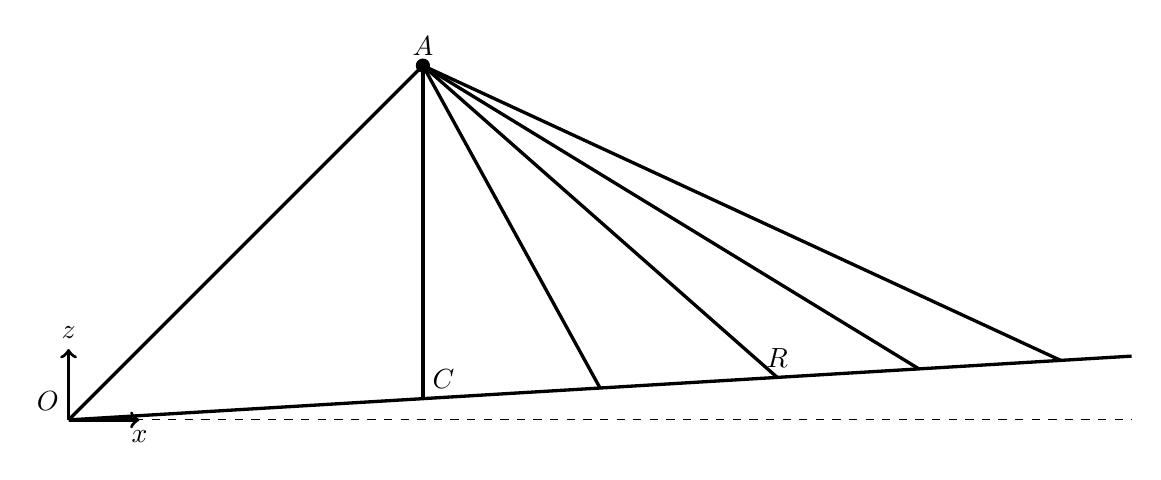
\begin{tikzpicture}[scale=0.9]
            \coordinate[label=above left:$O$] (O) at (0, 0);
            \coordinate[label=above:$A$] (A) at (5, 5);
            \coordinate[label=above right:$C$] (C) at (5, 0.3);
            \coordinate[label=above:$R$] (R) at (10, 0.6);

            \draw[very thick] (O) -- (15, 0.9);

            \fill (A) circle[radius=0.1];
            \draw[very thick] (O) -- (A);
            \draw[very thick] (A) -- (C);
            \draw[very thick] (A) -- (R);
            \draw[dashed] (O) -- (15, 0);
            
            \draw[very thick] (A) -- (7.5, 0.45);
            \draw[very thick] (A) -- (12, 0.72);
            \draw[very thick] (A) -- (14, 0.84);

            \draw[very thick, ->] (O) -- (1, 0) node[anchor=north] {$x$};
            \draw[very thick, ->] (O) -- (0, 1) node[anchor=south] {$z$};
        \end{tikzpicture}
    \end{center}

    \begin{enumerate}
        \item Find the Cartesian equation of the plane.
    \end{enumerate}

    Point $A$ is at the top of the vertical tower and has coordinates $(20, 1, 20)$. Point $C$ is the intersection of the tower and the deck. The tower and the five cables are attached on the deck along the line passing through Points $O$ and $C$.

    \begin{enumerate}
        \setcounter{enumi}{1}
        \item The bridge is considered stable if the distance between $C$ and the foot of perpendicular from $A$ to the deck does not exceed 1 m. Comment whether the bridge is stable. Show your working clearly.
        \item One of the cables, which is installed at a point $R$, has the same length as the main cable. Find the coordinates of $R$.
        \item Find the acute angle that the deck makes with the horizontal plane.
    \end{enumerate}
\end{problem}
\begin{solution}
    \begin{ppart}
        Observe that $\cveciiix{20}{0}1$ and $\cveciiix{40}{4}{2}$ are parallel to the plane. Note that \[\cveciii{20}{0}{1} \crossp \cveciii{40}{4}{2} = \cveciii{-4}{0}{80} \parallel \cveciii{-1}{0}{20}.\] Hence, the vector equation of the plane is \[\vec r \cdot \cveciii{-1}{0}{20} = 0,\] whence the Cartesian equation is $-x + 20 z = 0, y \in \RR$.
    \end{ppart}
    \begin{ppart}
        Observe that $\oa{AC} = k\cveciiix001$ for some $k \in \RR$. Hence, $\oa{OC} = \cveciiix{20}{1}{20-k}$. Since $C$ lies on the deck, we have \[\cveciii{20}{1}{20-k} \dotp \cveciii{-1}{0}{20} = 0,\] whence $k = 19$ and $\oa{OC} = \cveciiix{20}{1}{1}$.

        Let $F$ be the foot of perpendicular of $A$ to the deck. Note that $\oa{OF} \dotp \cveciiix{-1}{0}{20} = 0$ and $\oa{AF} = \l \cveciiix{-1}{0}{20}$ for some $\l \in \RR$. Thus, \[\bs{\cveciii{20}{1}{20} + \l\cveciii{-1}{0}{20}} \dotp \cveciii{-1}{0}{20} = 0, \implies \l = -\frac{380}{401} \implies \oa{OF} = \frac1{401} \cveciii{8400}{401}{420}.\] Hence, \[\oa{FC} = \cveciii{20}{1}{1} - \frac1{401} \cveciii{8400}{401}{420} \implies \abs{\oa{FC}} = \sqrt{0.948^2 + 0^2 + (-0.0474)^2} = 0.949 < 1.\] The bridge is thus stable.
    \end{ppart}
    \begin{ppart}
        We have $\abs{\oa{AR}} = \abs{\oa{OA}} = \sqrt{20^2 + 1^2 + 20^1} = \sqrt{801}$. Since $O$, $C$ and $R$ are collinear, we also have $\oa{OR} = \m \cveciiix{20}{1}{1}$ for some $\m \in \RR$. Thus, \[\abs{\oa{AR}} = \abs{\m \cveciii{20}{1}{1} - \cveciii{20}{1}{20}} = \sqrt{(20\m-20)^2 + (\m - 1)^2 + (\m - 20)^2} = \sqrt{801}.\] Using G.C., $\m = 2.09$, whence $R(41.9, 2.09, 2.09)$.
    \end{ppart}
    \begin{ppart}
        Let $\t$ be the acute angle between the deck and the horizontal. Note that the horizontal plane has normal vector $\cveciiix001$. Thus, \[\cos \t = \frac{\abs{\cveciiix001 - \cveciiix{-1}0{20}}}{\abs{\cveciiix001}\abs{\cveciiix{-1}0{20}}} = \frac{20}{\sqrt{401}} \implies \t = 2.9\deg \todp{2}.\]
    \end{ppart}
\end{solution}

\begin{problem}
    A nuclear reactor plant is built to meet the increased demand for electricity due to a particular country's economic developments. The cooling tower of the nuclear reactor is as shown in the figure below. The curved surface area of the cooling tower is modelled by rotating the region enclosed by a part of a hyperbolic curve about an axis. The height of the tower is 130 m.

    \begin{center}\tikzsetnextfilename{5}
        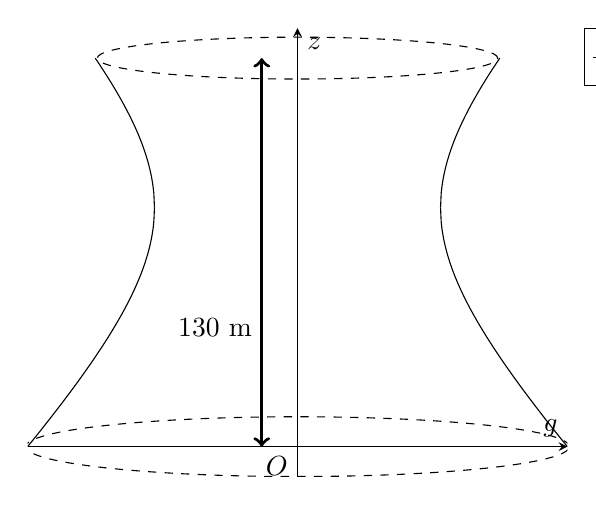
\begin{tikzpicture}[trim axis left, trim axis right]
            \begin{axis}[
                restrict y to domain = 0:130,
                samples = 201,
                ymax = 140,
                ymin = -10,
                axis y line=middle,
                axis x line=middle,
                xtick = \empty,
                ytick = \empty,
                xlabel = {$g$},
                ylabel = {$z$},
                legend cell align={left},
                legend pos=outer north east,
                after end axis/.code={
                    \path (axis cs:0,0) 
                        node [anchor=north east] {$O$};
                    }
                ]
                \addplot[black, domain=40:76] {sqrt(50^2 * (x^2 / 40^2 - 1)) + 80};
                \addplot[black, domain=40:76] {-sqrt(50^2 * (x^2 / 40^2 - 1)) + 80};
                \addplot[black, domain=-40:-76] {sqrt(50^2 * (x^2 / 40^2 - 1)) + 80};
                \addplot[black, domain=-40:-76] {-sqrt(50^2 * (x^2 / 40^2 - 1)) + 80};
    
                \addlegendentry{$\frac{g^2}{40^2} - \frac{(z-80)^2}{50^2} = 1$};

                \draw[dashed] (0, 0) ellipse[x radius=76, y radius=10];

                \draw[dashed] (0, 130) ellipse[x radius=56, y radius=7];

                \draw[very thick, <->] (-10, 0) -- (-10, 130);
                \node[anchor=east] at (-10, 40) {130 m};
    
            \end{axis}
        \end{tikzpicture}
    \end{center}

    The equation of the hyperbolic curve is given as $\frac{g^2}{40^2} - \frac{(z-80)^2}{50^2} = 1$ where $g$ is the axis that represents the ground and $z$ is the axis that represents the height of the reactor. The curve surface area of the tower is formed by rotating the region bounded by the hyperbolic curve, the line $z = 130$ and the $g$ axis about the $z$-axis by $\pi$ radians. The external curved surface area of the tower is to be painted with weather resistant paint.

    \begin{enumerate}
        \item Find the external curved surface area of the tower. Leave your answer to the nearest m$^2$.
    \end{enumerate}

    The ground is now represented by the $x$-$y$ plane.

    \begin{enumerate}
        \setcounter{enumi}{1}
        \item Find the Cartesian equation that models the surface of the tower in terms of $z$, $y$ and $z$.
    \end{enumerate}

    Before the paint can be applied, a robot is programmed to go around the tower to clean and polish its surface. Assuming that the robot is negligible compared to the tower, it can be viewed as a point on the curved surface of the tower.

    \begin{enumerate}
        \setcounter{enumi}{2}
        \item Given that the robot is at $(40, 40, 30)$ and is about the move in the direction of $\cveciix{3}{-4}$ parallel to the $x$-$y$ plane, determine whether the robot will be ascending or descending in height.
    \end{enumerate}

    The robot is now at $(40, 40, 130)$ on the surface of the tower. A signal needs to be transmitted from the ground to the robot such that the signal travels in a straight line and its direction must be normal to the surface of the tower where the robot is at.

    \begin{enumerate}
        \setcounter{enumi}{3}
        \item Find the coordinates on the ground where the signal can be transmitted to the robot.
    \end{enumerate}
\end{problem}
\begin{solution}
    \begin{ppart}
        Note that $g = \sqrt{40^2 \bs{\frac{(z-80)^2}{50^2} + 1}}$. Using G.C., \[\area = 2\pi \int_0^{130} g \sqrt{1 + \bp{\der{g}{z}}^2} \d z \approx 45552 \units[2].\]
    \end{ppart}
    \begin{ppart}
        For every constant value of $z$, we will have the value of $g$ such that $x^2 + y^2 = g^2$. Hence, \[\frac{x^2+y^2}{40^2} - \frac{(z-80)^2}{50^2} = 1.\]
    \end{ppart}
    \begin{ppart}
        Implicitly differentiating the above expressing with respect to $x$ and $y$, we have \[\pder{z}{x} = \bp{\frac54}^2 \frac{x}{z-80}, \quad \pder{z}{y} = \bp{\frac54}^2 \frac{y}{z-80}.\] Evaluating at $(40, 40, 30)$, we have that $\nabla z = -\frac54 \cveciix11$. Hence, \[\nabla z \cdot \frac1{\sqrt{3^2 + 5^2}} \cvecii3{-4} = \frac14 > 0.\] Thus, the robot is ascending.
    \end{ppart}
    \begin{ppart}
        At $(40, 40, 130)$, we have $\nabla z = \cveciix{5/4}{5/4}$. The equation of the tangent plane at that point is hence \[z = 130 + \frac54(x - 40) + \frac54(y - 40),\] which has vector equation \[\vec r \cdot \cveciii55{-4} = -120.\] The line of the signal is hence given by \[\vec r = \cveciii{40}{40}{130} + \l \cveciii55{-4}, \quad \l \in \RR.\] Setting $z = 0$, we have $\l = 130/4$, whence $x = y = 405/2$. The required coordinates are thus $\bp{\frac{405}2, \frac{405}2, 0}$.
    \end{ppart}
\end{solution}